\begin{exercise}
	Δίνονται τα σημεία $P_1 (3,5), P_2(7,7), P_3 (8,6)$. Θεωρώντας ότι το pixel που αντιστοιχεί στο $P_1(3,5)$ φωτίζεται στην οθόνη, να προσδιοριστούν στην οθόνη για τον σχεδιασμό των ευθυγράμμων τμημάτων $P_1 P_2, P_1 P_3$.

\begin{enumerate}
  \item[i)] Θεωρώντας ότι το pixel που αντιστοιχεί στο $P_1 (3,5) $ φωτίζεται στην οθόνη, να προσδιορισθούν οι συντεταγμένες των επόμενων pixels που θα φωτισθούν στην οθόνη για το σχεδιασμό των ευθυγράμμων τμημάτων $P_1 P_2, P_1 P _3$.
  \item[ii)]   Επιπλέον να μελετήσετε τον σχεδιασμό των ευθυγράμμων τμημάτων: \newline 
	$P_4 P_5, P_6 P_7, P_8 P_9, P_{10} P_{11}$.
\end{enumerate}

\begin{figure}[hbt]
  \begin{center}
	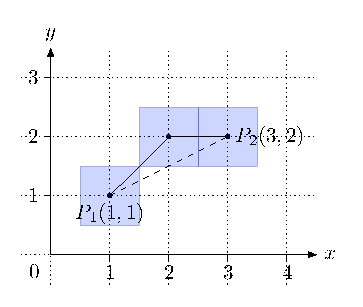
\includegraphics[scale=0.7]{Chapter1/Exercises/ex13/graph1.pdf}
  \end{center}
  \caption{Παράσταση ζητούμενων ευθυγράμμων τμημάτων}
\end{figure}


		
\end{exercise}

\begin{solution}

\begin{enumerate}
	
\item[i)] Γενικά ο αλγόριθμος του Bresenham για ευθείες στο πρώτο οκταμόριο είναι:

\begin{lstlisting}[caption={Αλγόριθμος του Bresenham για ζητούμενο ευθύγραμμο τμήμα}]
x1, y1 = get_coordinates("Give the coordinates of P1 e.g. (1,2):")
x2, y2 = get_coordinates("Give the coordinates of P2:")
Dx = x2 - x1
Dy = y2-y1
x = x1
y = y1
c1 = 2Dy
er = c1 - Dx
c2 = er - Dx
while x <= 7
    plot(x,y)
    x = x+1
    if er <0
        er = er + c1
    else
        y = y+1
        er = er + c2
    plot(x,y)
    end
end	
\end{lstlisting}

Για τα σημεία $P_1(3,5)$ και $P_2(7,7)$ θα έχουμε:

\begin{itemize}[noitemsep, topsep=0pt] % Reduce vertical spacing
\begin{multicols}{2} % Split into 2 columns
  \item $x = x_1 = 3$
  \item $y = y_1 = 5$
  \item $\Delta x = x_2 - x_1 = 5 - 3 = 4$
  \item $\Delta y = y_2 - y_1 = 7 - 5 = 2$
  \item $c_1 = 2 \cdot \Delta y = 2 \cdot 2 = 4$
  \item $er = c_1 - \Delta x = 4 - 4 = 0$
  \item $c_2 = er - \Delta x = 0 - 4 = -4$
\end{multicols}
\end{itemize}

Ο αλγόριθμος θα τρέξει ως εξής:

\lstset{style=tt} 
    
\begin{itemize}
  \item \underline{1η επανάληψη}

		\begin{lstlisting}
		x == 3 $<=$ 7 $\Rightarrow$
			plot(3,5) 
			x  = 4 %(x == x+1) 
			er == 0 $\geq$ 0 
				y = 6 %(y == y+1 == 6) 
				er = -4 %(er == er + c2 == 0 +(-4) == -4)
		\end{lstlisting}
		
	\item  \underline{2η επανάληψη}
		
		\begin{lstlisting}
		x == 4 $\leq$ 7 $\Rightarrow$
			plot(4,6)
			x = 5 %(x == x+1 == 5)
			er == -4 $<$ 0 $\Rightarrow$
				er = 0 %(er == er + c1 == -4 + 4 == 0)
		\end{lstlisting}		
				
	\item	\underline{3η επανάληψη}
		\begin{lstlisting}
		x == 5 $\leq$ 7 $\Rightarrow$
			plot(5,6)
			x = 6 %(x == x+1 == 6)
			er == 0 $\geq$ 0 $\Rightarrow$
				y = 7 %(y == y+1 == 7)
				er = -4 %(er == er + c2 == 0 +(-4) == -4)	
		\end{lstlisting}		
		
	\item	\underline{4η επανάληψη}
		\begin{lstlisting}
		x == 6 $\leq$ 7 $\Rightarrow$
			plot(6,7)
			x = 7 %(x == x+1 == 7)
			er == -4 $<$ 0 $\Rightarrow$
				er = 4 %(er == er + c1 == -4 + 4 == 0)		
		\end{lstlisting}
				
	\item	\underline{5η επανάληψη}
		\begin{lstlisting}
		x == 7 $\leq$ 7 $\Rightarrow$
			plot(7,7)
			x = 8 %(x == x+1 == 8)
			er == 4 $\geq$ 0 $\Rightarrow$
				y = 8 %(y == y+1 == 8)
				er = 8 %(er == er + c1 == 4 + 4 == 8)
		\end{lstlisting}
		
	\item	\underline{6η επανάληψη}
		\begin{lstlisting}
		x == 8 $>$ 7 $\Rightarrow$ %STOP
		\end{lstlisting}
\end{itemize}					


Συνολικά θα φωτιστούν τα σημεία : $(4, 6), (5, 6), (6, 7), (7,7)$.

Για τα σημεία $P_1(3,5)$ και $P_2(8,6)$ έχουμε:


\begin{itemize}[noitemsep, topsep=0pt] % Reduce vertical spacing
\begin{multicols}{2} % Split into 2 columns
  \item $x = x_1 = 3$
  \item $y = y_1 = 5$
  \item $\Delta x = x_2 - x_1 = 8 - 3 = 5$
  \item $\Delta y = y_2 - y_1 = 6 - 5 = 1$
  \item $c_1 = 2 \cdot \Delta y = 2 \cdot 1 = 2$
  \item $er = c_1 - \Delta x = 2 - 5 = -3$
  \item $c_2 = er - \Delta x = -3 - 5 = -8$
\end{multicols}
\end{itemize}


\begin{itemize}
\item \underline{1η επανάληψη}

\begin{lstlisting}
%Iteration 1:
x = 3 $\leq$ 8 $\Rightarrow$
    plot(3,5)
    x = 4 %(x = x+1 = 4)
    er = -3 < 0 $\Rightarrow$
        er = -1 %(er = er + c1 = -3 + 2 = -1)
    plot(4,5)
\end{lstlisting}

\item \underline{2η επανάληψη}

		\begin{lstlisting}
%Iteration 2:
x = 4 $\leq$ 8 $\Rightarrow$
    plot(4,5)
    x = 5 %(x = x+1 = 5)
    er = -1 < 0 $\Rightarrow$
        er = 1 %(er = er + c1 = -1 + 2 = 1)
    plot(5,5)
\end{lstlisting}

\item \underline{3η επανάληψη}

		\begin{lstlisting}
%Iteration 3:
x = 5 $\leq$ 8 $\Rightarrow$
    plot(5,5)
    x = 6 %(x = x+1 = 6)
    er = 1 >= 0 $\Rightarrow$
        y = 6 %(y = y+1 = 6)
        er = -7 %(er = er + c2 = 1 + (-8) = -7)
    plot(6,6)
\end{lstlisting}

\item \underline{4η επανάληψη}

		\begin{lstlisting}
%Iteration 4:
x = 6 $\leq$ 8 $\Rightarrow$
    plot(6,6)
    x = 7 %(x = x+1 = 7)
    er = -7 < 0 $\Rightarrow$
        er = -5 %(er = er + c1 = -7 + 2 = -5)
    plot(7,6)
\end{lstlisting}

\item \underline{5η επανάληψη}

		\begin{lstlisting}
%Iteration 5:
x = 7 $\leq$ 8 $\Rightarrow$
    plot(7,6)
    x = 8 %(x = x+1 = 8)
    er = -5 < 0 $\Rightarrow$
        er = -3 %(er = er + c1 = -5 + 2 = -3)
    plot(8,6)
\end{lstlisting}

\item \underline{6η επανάληψη}
\begin{lstlisting}
%Iteration 6:
x = 8 $\leq$ 8 $\Rightarrow$
    plot(8,6)
    x = 9 %(x = x+1 = 9)
    er = -3 < 0 $\Rightarrow$
        er = -1 %(er = er + c1 = -3 + 2 = -1)
    plot(9,6)
\end{lstlisting}

\end{itemize}

Συνολικά θα φωτιστούν τα σημεία : $(4, 5), (5, 5), (6, 6), (7,6), (8,6)$.	

\end{enumerate}
	
\end{solution}